\infolevone{

%  Re:  Hall C OPS Manual Chapter for DAQ and Trigger
% Date:  April, 2016

\par
The Hall C data acquisition uses CODA\cite{CODAwww}
(CEBAF Online Data Acquisition), a toolkit
developed at Jefferson Lab by the Data
Acquisition Group.

%For general information
%about CODA, see the
%CODA site\htmladdnormallinkfoot{}{\url{http://coda.jlab.org/}}.
%Up to date information about the Hall C DAQ
%is kept at
%\htmladdnormallinkfoot{}{\url{http://hallaweb.jlab.org/equipment/daq/daq_trig.html}}.

The signals from the photomultipliers and drift chambers are digitized
with high speed analog-to-digital converters (ADCs) and
time-to-digital converters (TDCs).  The digitizers currently in use
are:

\begin{list}{\arabic{enumi}.~}{\usecounter{enumi}\setlength{\itemsep}{-0.15cm}}
  \item CAEN V1190A TDCs \cite{V1190}.  These modules, with 128
    channels each, digitize discriminated signals with a resolution of
    100 ps.  They are used both for drift chambers and hodoscopes.
  \item FADC250 \cite{FADC250}.  These 16 channel ADC
    modules digitize the inputs with a 4 ns period.  When triggered
    they can provide either a digitized waveform, or an integrated
    amplitude.  Signals from the lead glass calorimeters, Cherenkov
    detectors and the hodoscopes are recorded with the FADC250s.
\end{list}

These modules are located in 5 VXS and VME64X crates located both in
the counting house electronics room and the detector/electronic
bunkers of the spectrometers.
\begin{itemize}
\item HMS Detector Hut: VXS crate with CAEN1190 TDCs for the HMS drift chambers
\item SHMS Electronics Hut:
\begin{itemize}
\item VME64X crate with CAEN1190 TDCs for the SHMS drift chambers
\item VXS crate with FADC250 modules for the SHMS Pre-shower and
shower detectors.
\end{itemize}
\item Counting House Electronics Room:
\begin{itemize}
\item VXS crate with FADC250 and CAEN1190 modules for the HMS
Hodoscopes, HMS Shower Counter and HMS Cherenkov detectors
and a Trigger Supervisor.
\item VXS crate with FADC250 and CAEN1190 modules for the SHMS
Hodoscopes, and Cherenkov detectors
and a Trigger Supervisor.
\end{itemize}
\end{itemize}

In addition to these crates, standard VME crates are for scalers.

This system of crates can be run as a single DAQ system for
coincidence experiments using both the HMS and SHMS.  Alternatively,
the system can be split into separate DAQ setups if one or both
spectrometers are being used for single arm measurements.

\par
The trigger supervisor is a custom--made
module built by the data
acquisition group.  Its functions are to
synchronize the readout crates, to administer
the deadtime logic of the entire system, and
to prescale various trigger inputs.
We have two trigger supervisors,
one in each spectrometer.  This allows us to
run the spectrometers independently if needed.

\par
The public account \mycomp{cdaq} is normally
used for running DAQ.  It is also used for online
analysis with the C++ analyzer \texttt{hcana} and online analysis software.
% Describe location of DAQ and analysis software.

%The trigger management software is run from the
%\mycomp{atrig} account and is described in
%the Trigger chapter.

% Somewhere describe how a run is started what settings
% (prescales and run conditions) need to be made

\section{Trigger Logic}
Each photomultiplier and drift chamber wire in the HMS and SHMS detectors
is digitized with a flash ADC, a TDC or both.  Many of these detectors are
used to make HMS, SHMS, or coincidence triggers, causing readout of these
digitized signals.  An block diagram overview of this DAQ/Trigger system is
show in Fig.~\ref{fig:trig_overview}.  Schematics for the electronics for
the various detectors are show in Figs.~\ref{fig:trig_hodoscopes},
\ref{fig:trig_hms_shower}, \ref{fig:trig_shms_preshower} and
\ref{fig:trig_aerogel_cherenkov}.

\begin{figure}
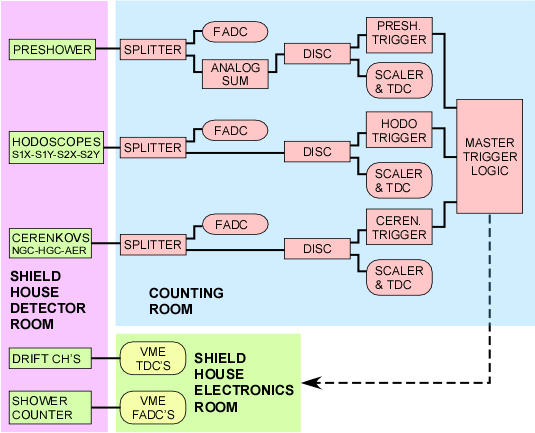
\includegraphics[width=6in]{trig_overview.png}
\caption{\label{fig:trig_overview}
Overview of the SHMS trigger and DAQ.  The HMS trigger is similar.
The HMS drift chamber TDCs are in the detector hut, while the Flash ADCs
for the HMS shower counter are located in the counting room.}
\end{figure}

\begin{figure}
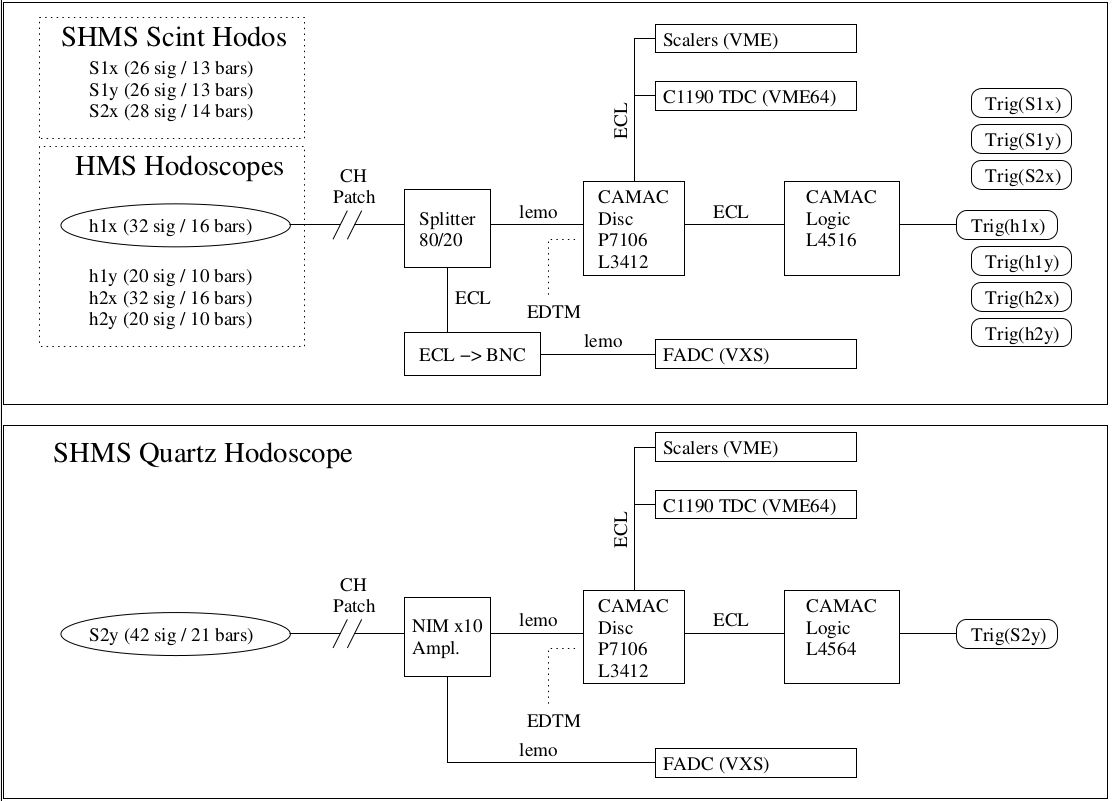
\includegraphics[width=6in]{trig_hodoscopes.png}
\caption{\label{fig:trig_hodoscopes}
Schematic of trigger and DAQ for the HMS and SHMS hodoscopes.  The CAMAC
L4564 modules are used to make logical ORs of each plane.  These OR'd signals
are then used, with other detectors, to make a user configurable event trigger.
}
\end{figure}

\begin{figure}
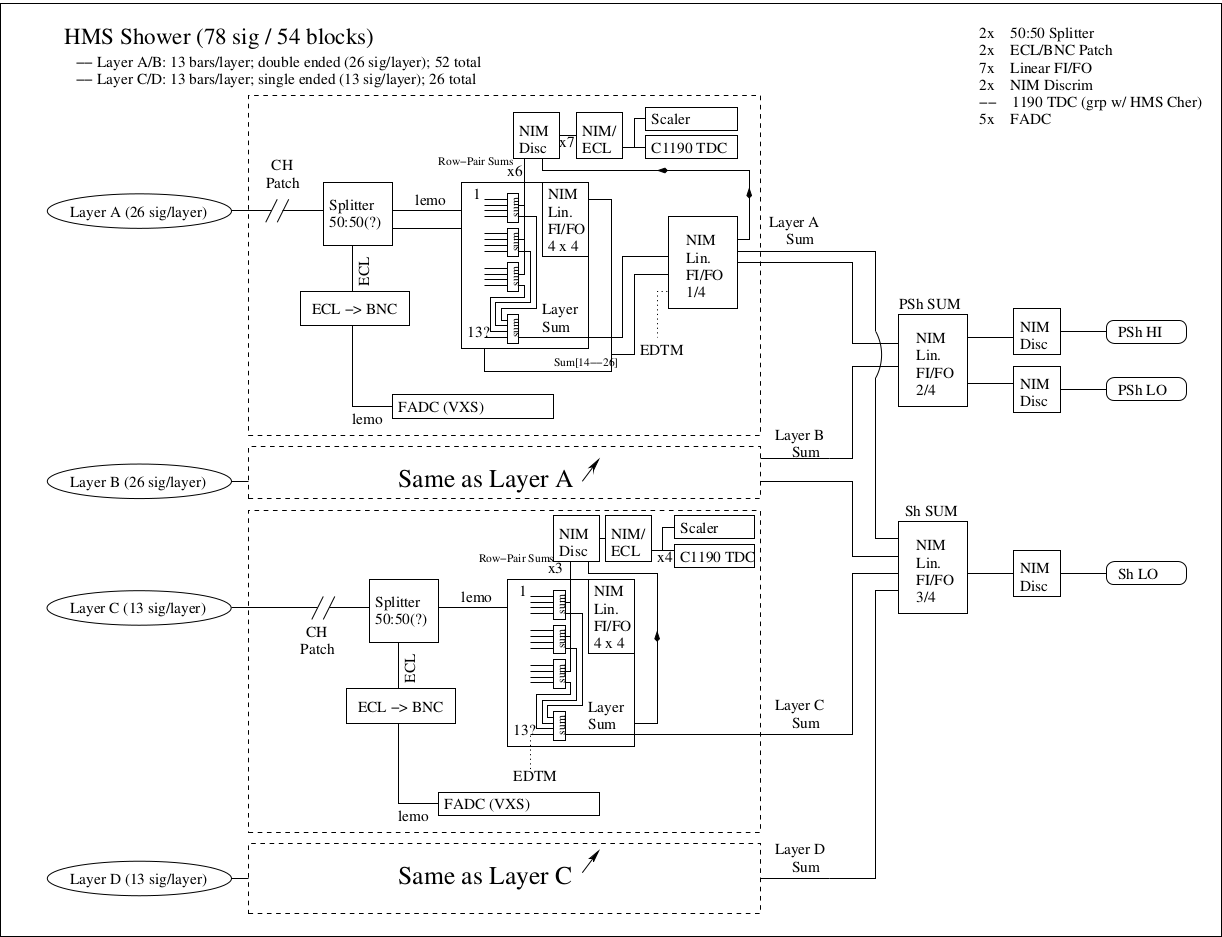
\includegraphics[width=6in]{trig_hms_shower.png}
\caption{\label{fig:trig_hms_shower}
Schematic of the HMS Shower counter DAQ and trigger.  The PSh HI, PSh LO,
and Sh LO signals are used, with other detectors, to make a user
configurable event trigger.
}
\end{figure}

\begin{figure}
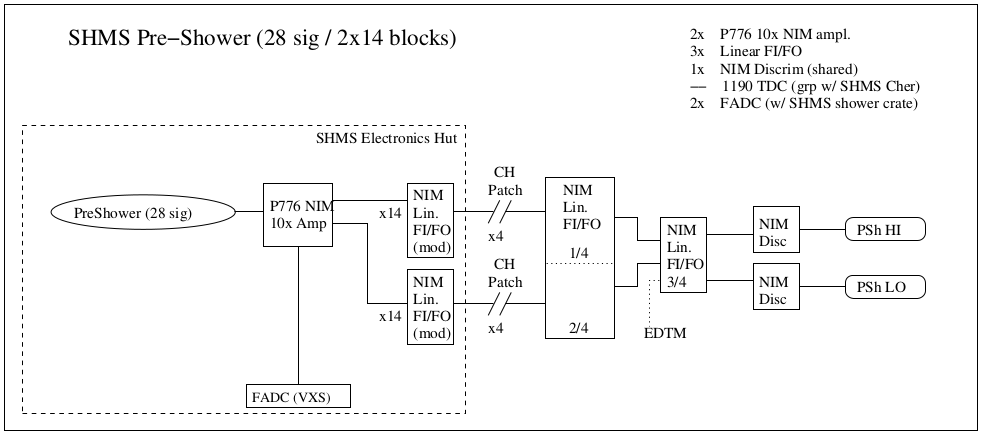
\includegraphics[width=6in]{trig_shms_preshower.png}
\caption{\label{fig:trig_shms_preshower}
Schematic of the DAQ and trigger for the SHMS Pre-Shower layer of the
SHMS shower detector.  The
PSh HI and PSh LO signals are used, with other detectors, to make a user
configurable event trigger.  The flash ADCs for the the 224 shower counter
blocks behind the pre-shower are also located in the SHMS Electronics Hut.
These blocks are not used in the trigger.
}
\end{figure}

\begin{figure}
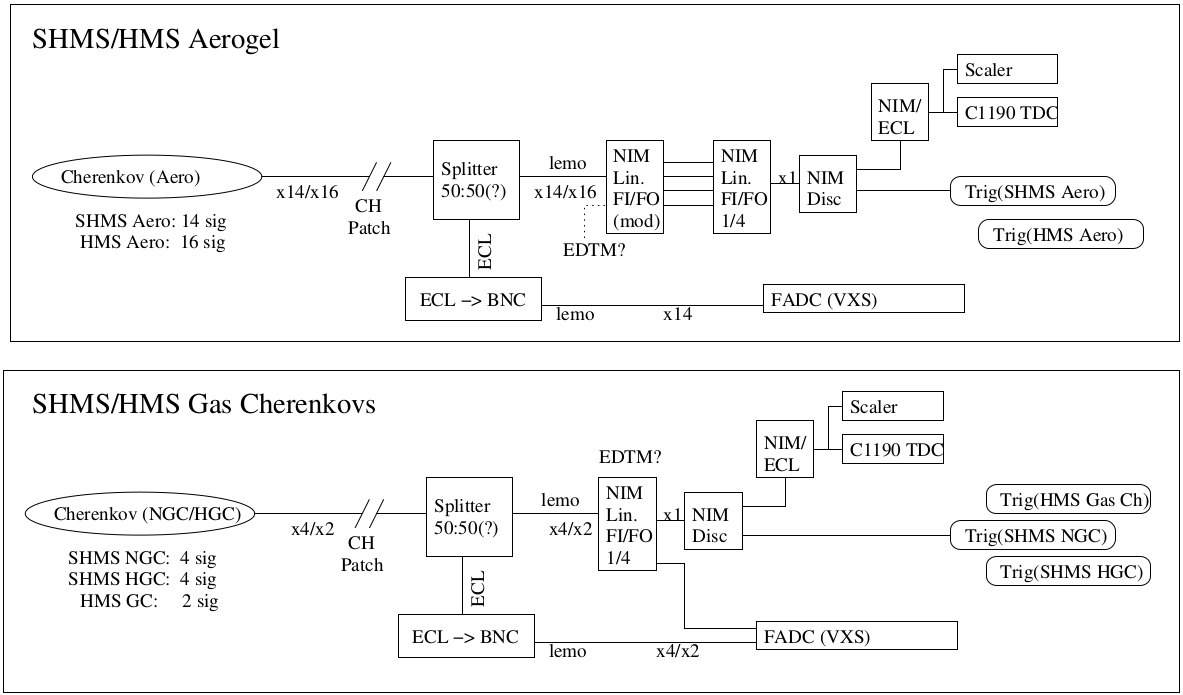
\includegraphics[width=6in]{trig_aerogel_cherenkov.png}
\caption{\label{fig:trig_aerogel_cherenkov}
Schematic of the DAQ and trigger for the Aerogel and Gas Cherenkov
detectors in the HMS and SHMS.  The Trig signals (SHMS Aero, HMS Aero,
HMS Gas CH, SHMS NGC, and SHMS HGC) are used, with other detectors, to
make a user configurable event trigger.
}
\end{figure}


\obsolete{ % Comment out until updated for Hall C
%\infolevtwo{

\section{General Computer Information}

\par
In the counting room we have various computers
for DAQ, analysis, and controls.  (Control systems are described
in Chapter~\ref{chap:controls}.)
The DAQ computer's names are denoted by \mycomp{cdaqlN} and \mycomp{hcdeskN},
where N is a number.
%  adaql1 and l2 are Linux computers for
%running DAQ while \mycomp{adaql3,4}... and higher
%are for analysis. A new computer has been installed and will be used for the
%Left HRS DAQ it is named adaq1 we plan to have adaq2 installed for Right HRS soon.
%The Linux PCs are administered mostly by Ole Hansen.

\par
To reboot the Linux machines, first hit \mycomp{Ctrl-Alt-F1}
to switch to a text console, then hit \mycomp{Ctrl-Alt-Del}
to reboot.
If power fails for a prolonged time,
you must shutdown before the UPS fails.


%\section{DAQ checklist}
%Things to check before experiment starts
%\begin{enumerate}
%\item blaster test transfer rate
%\item BPM cabling
%\item BCM cabling
%\item timestamp cabling
%\item raster cabling
%\item check portservers
%\item check reset
%\item check trigger latch is connected
%\item helicity if needed
%\item scalers
%\item synchronization time stamp
%\end{enumerate}
% A list should be in the section below



\section{Beginning of Experiment Checkout}

\par
This section describes the
checkout of DAQ and trigger
needed before an experiment can start.

\begin{enumerate}
\item{First ensure that all the fastbus, VME,
CAMAC, and NIM crates are powered
on. They should
boot up in a functional state, except for
heavily loaded fastbus crates that sometimes
lose their NVRAM.  (If that happens, see notes
in \mycomp{/adaqfs/halla/a-onl/doc/vmeram.doc}).}

%\item{You may download
%a default trigger, following the directions in
%the trigger chapter.  If the hadron momentum changes
%you may need to set a new delay.  A trigger expert
%should do the start-of-experiment
%trigger checklist.}

\item{Make sure the HV is on for all detectors
and that the values are normal.}

\item{Start the \mycomp{xscaler}
display following the instructions below and
check that the rates from detectors are normal.}

\item{Startup \mycomp{runcontrol} (CODA) using the directions below
and start a run.  With the trigger downloaded
and the HV on, you are taking cosmics data, typically at
a rate of 3 Hz per spectrometer.
Examine the data using ESPACE or the C++ analyzer.
Compare the plots and printouts to normal values.}

\end{enumerate}

\section{Running CODA}

\par
This section describes how to run CODA for
the spectrometer DAQ.  There are two modes:
(1) The most common is the ``1-Trigger-Supervisor (1-TS)''
mode which uses one trigger supervisor and
is used for coincidence experiments; and
(2) The ``2-Trigger-Supervisor (2-TS)'' mode which
is used for running the two spectrometers
independently.

\par
The 1-TS mode can also handle single--arm
triggers but is about 1/2 the aggregate speed
of the 2-TS mode.  When running the 2-TS
mode, one uses the adaq account on \mycomp{adaql2} or \mycomp{adaq1}  for one
spectrometer and the adev account on \mycomp{adaql1} or \mycomp{adaq2}
for the other spectrometer.
The 1-TS mode normally uses the
adaq account on \mycomp{adaql2} or \mycomp{adaq1}  only.
The information that follows refers to
the adaq account, but the other account is quite similar.

\par

Here is how to start and stop a run.
Normally, when you come on shift,
runcontrol will be running.  If not,
see the section on ``Cold Start'' below.
To start and stop runs, push the buttons
``Start Run'' and ``End Run'' in the
runcontrol GUI.   To change configurations
use the ``Run Type'' button.  If you have
been running you will first have to push the
``Abort'' button before you can change the
run type. Typically the configurations
you want are the following.

\begin{itemize}
\item[~]TWOSPECT -- For running the two spectrometers in
1-TS mode.
\item[~]PEDRUN -- To do a pedestal run in 1-TS mode
\item[~]RIGHTHRS -- For R-arm in 2-TS mode
\item[~]LEFTHRS -- For L-arm in 2-TS mode
\item[~]PEDRUNR -- To do a pulser run for R-arm in 2-TS mode
\item[~]PEDRUNL -- To do a pulser run for L-arm in 2-TS mode
\end{itemize}

\par
A note about pedestal runs.  They have the exclusive
purpose of obtaining pedestals used for pedestal
suppression.  For details about what is done
and hints for getting pedestals for analysis (which
does not want the PEDRUN result), see \mycomp{/ped/README}.

}
\obsolete{ % Comment out until adjusted for Hall C
%\infolevthree{

\subsection{
 Some Frequently Asked Questions about DAQ}


\begin{itemize}
\item{ {\it Q: Where is the data ?} \hskip 0.05in
Use a command ``find\_run 1745'' to find
where run 1745 has been written on disk and MSS.
The data are first written to disks like
\mycomp{/adaql2/dataN}, N=1,2,3...etc.  Files are
automatically split if they become bigger than a
prescribed limit, the split files have
suffixes .0,.1,.2...etc.
Files are archived automatically to tape in the MSS
tape silo.  Two tape copies are made.  Data are
purged from disk automatically.  Users should
{\it never} attempt to copy, move, or erase data.}

\item{ {\it Q: How to adjust prescale factors ? }
\hskip 0.05in
Edit the file \mycomp{\~/prescale/prescale.dat}.
One common problem is putting typographical
errors here which then leads to no triggers
getting accepted.}

\item{ {\it Q: What is the deadtime ? } \hskip 0.05in
The deadtime is displayed in the datamon
window, which normally is running next to the
runcontrol window, but if this window is
not up, type \mycomp{datamon} to bring it up.
This window also shows the full-path-name of the file
being written by CODA for the present run.}

\item{ {\it Q: Where are the crates ?} \hskip 0.05in
R-HRS has fastbus crates ROC1, ROC2, ROC7 on the lower level
of the detector hut, and a 9U (tall) VME crate TS0 on
the upper level.  L-HRS has fastbus ROC3, ROC4, ROC8 and
VME crate TS11.}

\item{ {\it Q: Why is the deadtime so high ?
(and related)} \hskip 0.1in
Search for answers among the following.
The standard lore is that 20\% deadtime is tolerable,
but you should ask your analysis team to decide.
Sometimes people seeing large deadtimes
have forgotten to observe that the beam is in
pulsed mode.  Another possibility is that the
workstation is overloaded.  The computer used
for CODA should not be used for anything else.
Do not attempt to read or write rapidly to the
same physical disk to which CODA is writing.
Sometimes it is observed that the workstation
itself is very sluggish.
This could be due to a foreign
mounted disk having gone away, and there are
other possible reasons.  If a Cold Start of CODA
doesn't solve the problem, you may
try rebooting the workstation
(see computer section).  Also, if
the event size changes substantially, e.g. due
to VDC or FPP thresholds being turned off (a common mistake),
the deadtime as a function
of rate will change, especially
in the regime of high rates.}

\end{itemize}

\subsection{ Quick Resets }

Problems with CODA can usually be solved with a simple
reset.  If not, try a Cold Start (see next section).
Do not waste an hour of beam time on resets;
if they fail, call an expert.
The expert claims he can restart CODA
90\% of the time within 10 minutes.

If a ROC (ReadOut Controller, or crate)
is hung up, reboot by going the workspace
``Components'' and typing \mycomp{reboot}.  If this
doesn't work, try pressing the reset button
which is on the ``Crate Resets'' section of the
Hall A General Tools EPICS~\cite{EPICSwww} Gui.
If this still fails for the FastBus crates there is a power cycle relay
which can be activated with the EPICS button : Fastbus Power AC.
 Telnet back into
the ROC to verify its alive.
If all failed call an expert and most likely an access will be needed.
Then press ``Reset''
in runcontrol, download and start a new run.

\subsection{ Cold Start of CODA}

\par
If CODA is not running, or if it gets hung up,
you can do a cold start.  Frequently a subset of
these steps is sufficient to recover from a hangup,
but it takes some experience to realize the
minimum of steps that
are necessary, so the simplest
thing is to do them all, which takes a few minutes.

\begin{itemize}
\item{Make sure the fastbus and VME crates are
running.  The crates are usually known by
``ROCnumber-computer-(portserver-port)''
where ROCnumber is the unique number for that
ROC (ReadOut Controller, or crate),
computer is the internet name and the
portserver-port is the portserver IP and port\#
where to login.
An example might be \hskip 0.05in
ROC4-hallasfi4-(hatsv4,port3) which is
ROC4, a fastbus crate with IP \mycomp{hallasfi4} attached
to the portserver IP \mycomp{hatsv4} at port 3.
You would telnet in with the command ``telnet hatsv4 2003''.
You can check if the ROCs
are up by looking on the Components work space
at the telnet session (if it's not logged,
try to telnet in).
If the ROCs don't talk to runcontrol, you can type
\mycomp{reboot} at the arrow prompt ($\rightarrow$).   If you
don't get this arrow prompt, or if you can't telnet in,
the computer is hung up, so press
the reset button in the ``Crate Resets'' GUI
available from the EPICS screen for
Hall A General Tools.
After the ROC comes back (2 minutes),
telnet back in to verify it's up.
On rare occasions it is necessary to
power cycle the crate, which requires access. }
\item{ Start runcontrol and the other necessary
processes by typing \mycomp{startcoda}.  Note,
\mycomp{startcoda} first cleans up old processes
for you, so you don't need to take care of that.}
\item{ In runcontrol,
press the ``Connect'' button.
Wait 5 seconds and press ``Run Types''.
After configure and before download,
press the ``Reset'' button in the upper left corner.
Choose the run type from the dialog box
(see section on Running
CODA for descriptions of run types).}
\item{ After you configure and download the Run Type,
you can ``Start Run'' to start a new run.}


\end{itemize}


\subsection{ Recovering from a Reboot of Workstation}

If the workstation from which you are running CODA
was rebooted, here is how to recover DAQ.
Login as the relevant account, which is usually
a-onl for 1-DAQ operation. Passwords for the online
accounts should be available on a paper on the wall
in the counting room, or ask the run coordinator.
In the workspace for ``Components'' telnet into
all the ROCs.  If the x-terms windows are not
available, type \mycomp{setupxterms}.  Start emacs
for the prescale factors:
\mycomp{emacs /prescale/prescale.dat}.
Make sure msqld is running in the process list;
it is supposed to start when the computer boots.
Then do a Cold Start (see section above).

}
\obsolete{ % Comment out until adjusted for Hall C
%\infolevone{

\section{Electronic Logbook and Beam Accounting}

Two major tools are available for logging information
by the shift workers: \hskip 0.05in
(1) The Electronic Logbook ``hclog'', and
\hskip 0.05in
(2) The Hall Beam--Time Accounting tool.

\par
The electronic logbook is a web-based
repository of logbook data available at
\url{https://logbooks.jlab.org/book/hcloghttps://logbooks.jlab.org/book/hclog}.
There are
several ways to make entries:  One can use
the hclog GUI (type \mycomp{hclog} and make your
entry), or one may use a script
to insert a file.
Some data from EPICS
and scalers, among other things, are inserted
automatically into hclog on each start-of-run
and each end-of-run.  These data also get
written into files with the run number in
their name in \mycomp{/epics/runfiles}.
Data appear on the web at a certain URL
\htmladdnormallinkfoot{}{\url{http://www.jlab.org/~adaq/halog/html/logdir.html}}.
It is recommended that one software expert
from the experiment be
assigned to modify the logging scripts
as he or she sees fit.

\par
The Hall Beam--Time Accounting Table is the mechanism
to summarize and record
how the beam time in a shift was spent.
The shift leader is responsible for
submitting this table at the end of the shift.
When submitted, the data are
logged in a database
and a summary is e-mailed to various people like the
run coordinators and the hall leader.
When you come on shift, the GUI is probably
already running.  If not, you may start it
by logging onto \mycomp{adaql1} as the
adaq account and type ``\mycomp{bta}''.
It is a fairly obvious GUI,
but there is also some online help.

}
\obsolete{ % Comment out until adjusted for Hall C
%\infolevthree{

\section {Port Servers}
Portservers are devices on the network that
allow access to RS232 ports (see Table \ref{tab:daq:portservers}).
  Here is how to
connect from a computer: \mycomp{telnet hatsv5 2011}
will connect to the portserver at IP \mycomp{hatsv5}
and port 11.  Note, the offset of 2000 is needed.
For dealing with HV, it is best to use a Linux PC
for which the keymap is F1 = PF1 and F2 = PF2.

If another person is connected to a certain port,
you cannot connect.  To bump off another user, login
as root with password available from the paper posted
on the wall of the counting room (or ask run coordinator)
as follows \mycomp{telnet hatsv5} as user = root.
At the prompt, type \mycomp{kill tty=4} to clear port 4,
then \mycomp{exit}.  Now you can \mycomp{telnet hatsv5 2004}.


} %infolev

\infolevltone{\newpage}
\begin{safetyen}{10}{15}
\section{Authorized  Personnel}
\end{safetyen}
The authorized personnel is shown in table \ref{tab:daq:personnel}.
\begin{namestab}{tab:daq:personnel}{DAQ: authorized personnel}{%
      DAQ: authorized personnel.}
%  \StephenWood{}
  \RobertMichaels{}
  \OleHansen{Computers}
\end{namestab}

\obsolete{  % Comment out until adjusted for Hall C
%\infolevthree{
\begin{table}[htp]
\centering
\begin{tabular}{|l|l|l|}  \hline
server IP &  Port & Device \\ \hline
\mycomp{hatsv3}    &   1     &  vt100 Dumb Terminal \\
\mycomp{hatsv3}    &   2     &  ROC1 Lower Fastbus Crate \\
\mycomp{hatsv3}    &   3     &  TS0 Trig. Super. VME Crate \\
\mycomp{hatsv3}    &   4     &  R-arm Upper HV Crate \\
\mycomp{hatsv3}    &   5     &  R-arm Lower HV Crate \\
\mycomp{hatsv3}    &   8     &  ROC2 Upper Fastbus Crate \\
\mycomp{hatsv4}    &   1     &  vt100 Dumb Terminal \\
\mycomp{hatsv4}    &   2     &  ROC3 Lower Fastbus Crate \\
\mycomp{hatsv4}    &   3     &  ROC4 Upper Fastbus Crate \\
\mycomp{hatsv4}    &   5     &  HV Crate   \\
\mycomp{hatsv4}    &   6     &  RICH HV Crate \\
\mycomp{hatsv4}    &   7     &  RICH VME Crate \\
\mycomp{hatsv4}    &   14    & TS1 Trig. Super. VME Crate \\
\mycomp{hatsv5}    &   1     &  vt100 Dumb Terminal \\
\mycomp{hatsv5}    &   2     &  e-P Crate 1 \\
\mycomp{hatsv5}    &   3     &  Moller 1 \\
\mycomp{hatsv5}    &   4     &  Moller 2 \\
\mycomp{hatsv5}    &   8     &  Compton ROC3 \\
\mycomp{hatsv5}    &   9     &  Compton ROC4 \\
\mycomp{hatsv5}    &   10    &  Compton ROC5 \\
\mycomp{hatsv5}    &   11    &  Beamline HV  \\
\mycomp{hatsv5}    &   12    &  e-P Crate 2 \\
\mycomp{hatsv5}    &   13    &  ARC Energy \\
\mycomp{hatsv5}    &   14    &  ROC14 VME Crate \\
\mycomp{hatsv5}    &   15    &  ROC15 VME Crate \\
\mycomp{hatsv12}   &   5     &  Compton ROC1 \\
\mycomp{hatsv12}   &   6     &  Compton ROC2 \\
\mycomp{hatsv15}   &   -     &  2nd Floor Counting Room \\
\mycomp{hatsv9}    &   4     &  Parity DAQ Crate \\
\hline
\end{tabular}
\caption[Data Acquisition: Port Servers for DAQ]{
Port Servers for DAQ}
\label{tab:daq:portservers}
\end{table}
} %infolev
}
